\documentclass[11pt,a4paper]{article}

\usepackage[utf8]{inputenc}
\usepackage[T1]{fontenc}
\usepackage[french]{babel}
\usepackage{lmodern}
\usepackage[margin=2.3cm]{geometry}
\usepackage{setspace}
\usepackage{parskip}
\usepackage{titlesec}
\usepackage{fancyhdr}
\usepackage{graphicx}
\usepackage{array}
\usepackage{booktabs}
\usepackage{tabularx}
\usepackage{longtable}
\usepackage{xcolor}
\usepackage[hidelinks,
            colorlinks=true,
            linkcolor=black,
            urlcolor=blue!60!black,
            citecolor=black]{hyperref}
\usepackage{enumitem}
\setlist[itemize]{itemsep=2pt,topsep=4pt}

\setlength{\headheight}{1cm}
\pagestyle{fancy}
\fancyhf{}
\fancyhead[L]{Hubble Lakehouse --- Rapport}
\fancyhead[R]{
\includegraphics[height=0.7cm]{logo.png}}
\fancyfoot[C]{\thepage}
\renewcommand{\headrulewidth}{0.4pt}

\title{Hubble Lakehouse \\[0.3cm]
       \large Rapport \\[0.2cm]
       \normalsize Pipeline Big Data pour l'analyse des observations du télescope spatial Hubble}
\author{Valentin Massonnière \and Kevin Heugas}
\date{\today}

\begin{document}

\begin{titlepage}
    \centering
    \vspace*{1cm}

    
\includegraphics[width=4cm]{logo.png}\\[1cm]

    {\Large \textbf{EFREI Paris}}\\[0.3cm]
    {\large Formation \textit{Big Data Framework}}\\[3cm]

    \rule{\linewidth}{0.5pt}\\[0.6cm]
    {\Huge \textbf{Hubble Lakehouse}}\\[0.4cm]
    {\LARGE Rapport}\\[0.6cm]
    {\large Pipeline Big Data pour l'analyse des observations\\ du télescope spatial Hubble}\\[0.4cm]
    \rule{\linewidth}{0.5pt}\\[2.5cm]

    {\large \textbf{Auteurs}}\\[0.4cm]
    {\large Valentin Massonnière}\\
    {\large Kevin Heugas}\\[3cm]

    {\large \today}

    \vfill
\end{titlepage}

\tableofcontents
\newpage

\paragraph{Note méthodologique.} Ce rapport a d'abord été rédigé en brouillon par nous-mêmes. Une IA nous a aidé à nous corriger les fautes et reformuler certaines phrases, sans modifier les justifications ni ajouter de contenu. L'objectif est de gagner du temps de rédaction et de limiter les fautes.

\newpage

% ----------- PARTIE 1 -------------
\section{Introduction}

\subsection{Contexte}

Lancé en 1990 par la NASA et l'ESA, le télescope spatial Hubble (HST) constitue depuis plus de 30 ans l'un des instruments scientifiques le plus puissant de l'histoire de l'astronomie. Ses observations couvrent un large spectre, de l'ultraviolet au proche infrarouge, et alimentent des champs de recherche aussi variés que la cosmologie, l'étude des exoplanètes ou la physique stellaire.

L'ensemble des observations produites par Hubble est mis à disposition du public via deux archives principales : le \href{https://mast.stsci.edu/portal/Mashup/Clients/Mast/Portal.html}{\textit{Mikulski Archive for Space Telescopes}} (MAST) opéré par le STScI, et l'\href{https://www.cosmos.esa.int/web/hst/fetching-data}{\textit{ESA Hubble Science Archive}} opéré par l'ESAC.

\subsection{Objectifs du projet}

Le projet vise à concevoir, implémenter et documenter une \textbf{architecture Lakehouse complète} suivant la logique \textit{Médaillon} (couches Bronze, Silver, Gold), capable de :

\begin{itemize}
    \item \textbf{Ingérer} de manière fiable deux sources hétérogènes : un historique massif d'observations Hubble (batch) et un flux continu de météo spatiale (streaming) ;
    \item \textbf{Stocker} la donnée brute dans un système de fichiers distribué (HDFS) sans transformation préalable, garantissant rejouabilité et auditabilité ;
    \item \textbf{Nettoyer, typer et structurer} la donnée dans une couche intermédiaire (Hive / Parquet) servant de socle commun à l'ensemble des cas d'usage ;
    \item \textbf{Modéliser et matérialiser} dans une base relationnelle (PostgreSQL) quatre datamarts métier répondant à des problématiques scientifiques et techniques concrètes ;
    \item \textbf{Tracer} chaque étape du pipeline par des logs consultables depuis le dashboard Airflow.
\end{itemize}

\subsection{Livrables attendus}

Les livrables attendus sont :

\begin{itemize}
    \item un \textbf{rapport écrit} décrivant l'architecture, les choix techniques, les jeux de données mobilisés et les résultats obtenus ;
    \item un \textbf{dépôt GitHub} regroupant l'ensemble du code source du pipeline.
\end{itemize}

\newpage
% ----------- PARTIE 2 -------------
\section{Périmètre fonctionnel}

\subsection{Profils utilisateurs}

Le projet répond à quatre problématiques posées par quatre métiers scientifiques.

\paragraph{Physicien.} Quelles régions du ciel ont été sur-observées par Hubble, et quels sont les angles morts de la recherche~?

\paragraph{Chimiste.} Quelles cibles ont été observées avec des filtres à bande étroite correspondant à des raies d'émission spécifiques (H$\alpha$, OIII, SII\dots)~?

\paragraph{Biologiste.} Quelles observations ont été acquises pendant une éruption solaire ou un événement de météo spatiale, et risquent d'être corrompues par les radiations~?

\paragraph{Ingénieur spatial.} Comment évoluent les temps de calibration des instruments Hubble au fil du temps~?

\subsection{Hors-périmètre}

Le projet ne couvre pas :

\begin{itemize}
    \item l'analyse du contenu des images FITS ; seules les métadonnées sont exploitées ;
    \item la prédiction (apprentissage automatique) ; les datamarts servent au reporting et à l'exploration ;
\end{itemize}

\newpage
% ----------- PARTIE 3 -------------
\section{Sources de données}

\subsection{Source 1 --- MAST}

MAST est l'archive publique des observations Hubble, accessible via le \href{https://mast.stsci.edu/portal/Mashup/Clients/Mast/Portal.html}{portail web} du STScI. Les métadonnées sont exportées au format CSV. Le fichier utilisé contient environ 500\,000 lignes, décrites par le schéma CAOM (\textit{Common Archive Observation Model}).

Pour répondre à l'obligation pédagogique d'avoir une base de données en source, le fichier CSV est chargé tel quel dans une table PostgreSQL dédiée au démarrage du projet. C'est cette table qui est ensuite consommée par le pipeline d'ingestion vers Bronze, et non le fichier CSV brut.

\subsection{Source 2 --- NOAA SWPC}

NOAA SWPC publie en quasi-temps réel les indicateurs de météo spatiale : vent solaire, flux X-ray, indice planétaire Kp, éruptions solaires. Les données sont disponibles au format JSON sur des endpoints HTTP (\href{https://services.swpc.noaa.gov/json/}{services.swpc.noaa.gov/json/}), la récupération se fait en mode streaming.

\subsection{Choix des sources}

MAST fournit un historique statique traité en batch. NOAA SWPC fournit un flux temps réel traité en streaming.

\subsection{Synchronisation temporelle des sources}

Les deux sources ne couvrent pas le même horizon temporel. MAST contient des observations qui s'étalent sur plus de trente ans, alors que les endpoints JSON de NOAA SWPC n'exposent que les indicateurs récents (quelques jours à quelques semaines selon le produit). Sans correction, le datamart Biologiste ne pourrait croiser les éruptions solaires qu'avec les rares observations Hubble réalisées pendant la fenêtre courante du flux SWPC.

Pour lever cette limite, les archives historiques de NOAA SWPC sont récupérées en amont puis chargées dans Bronze en complément du flux temps réel. 
\newpage
% ----------- PARTIE 4 -------------
\section{Architecture}

\subsection{Vue d'ensemble}

L'architecture suit le patron Médaillon, organisé en trois couches successives : Bronze, Silver et Gold. Les données circulent des sources jusqu'aux outils de restitution en passant par chacune de ces couches. La figure~\ref{fig:archi} présente le pipeline complet.

\begin{figure}[h!]
    \centering
    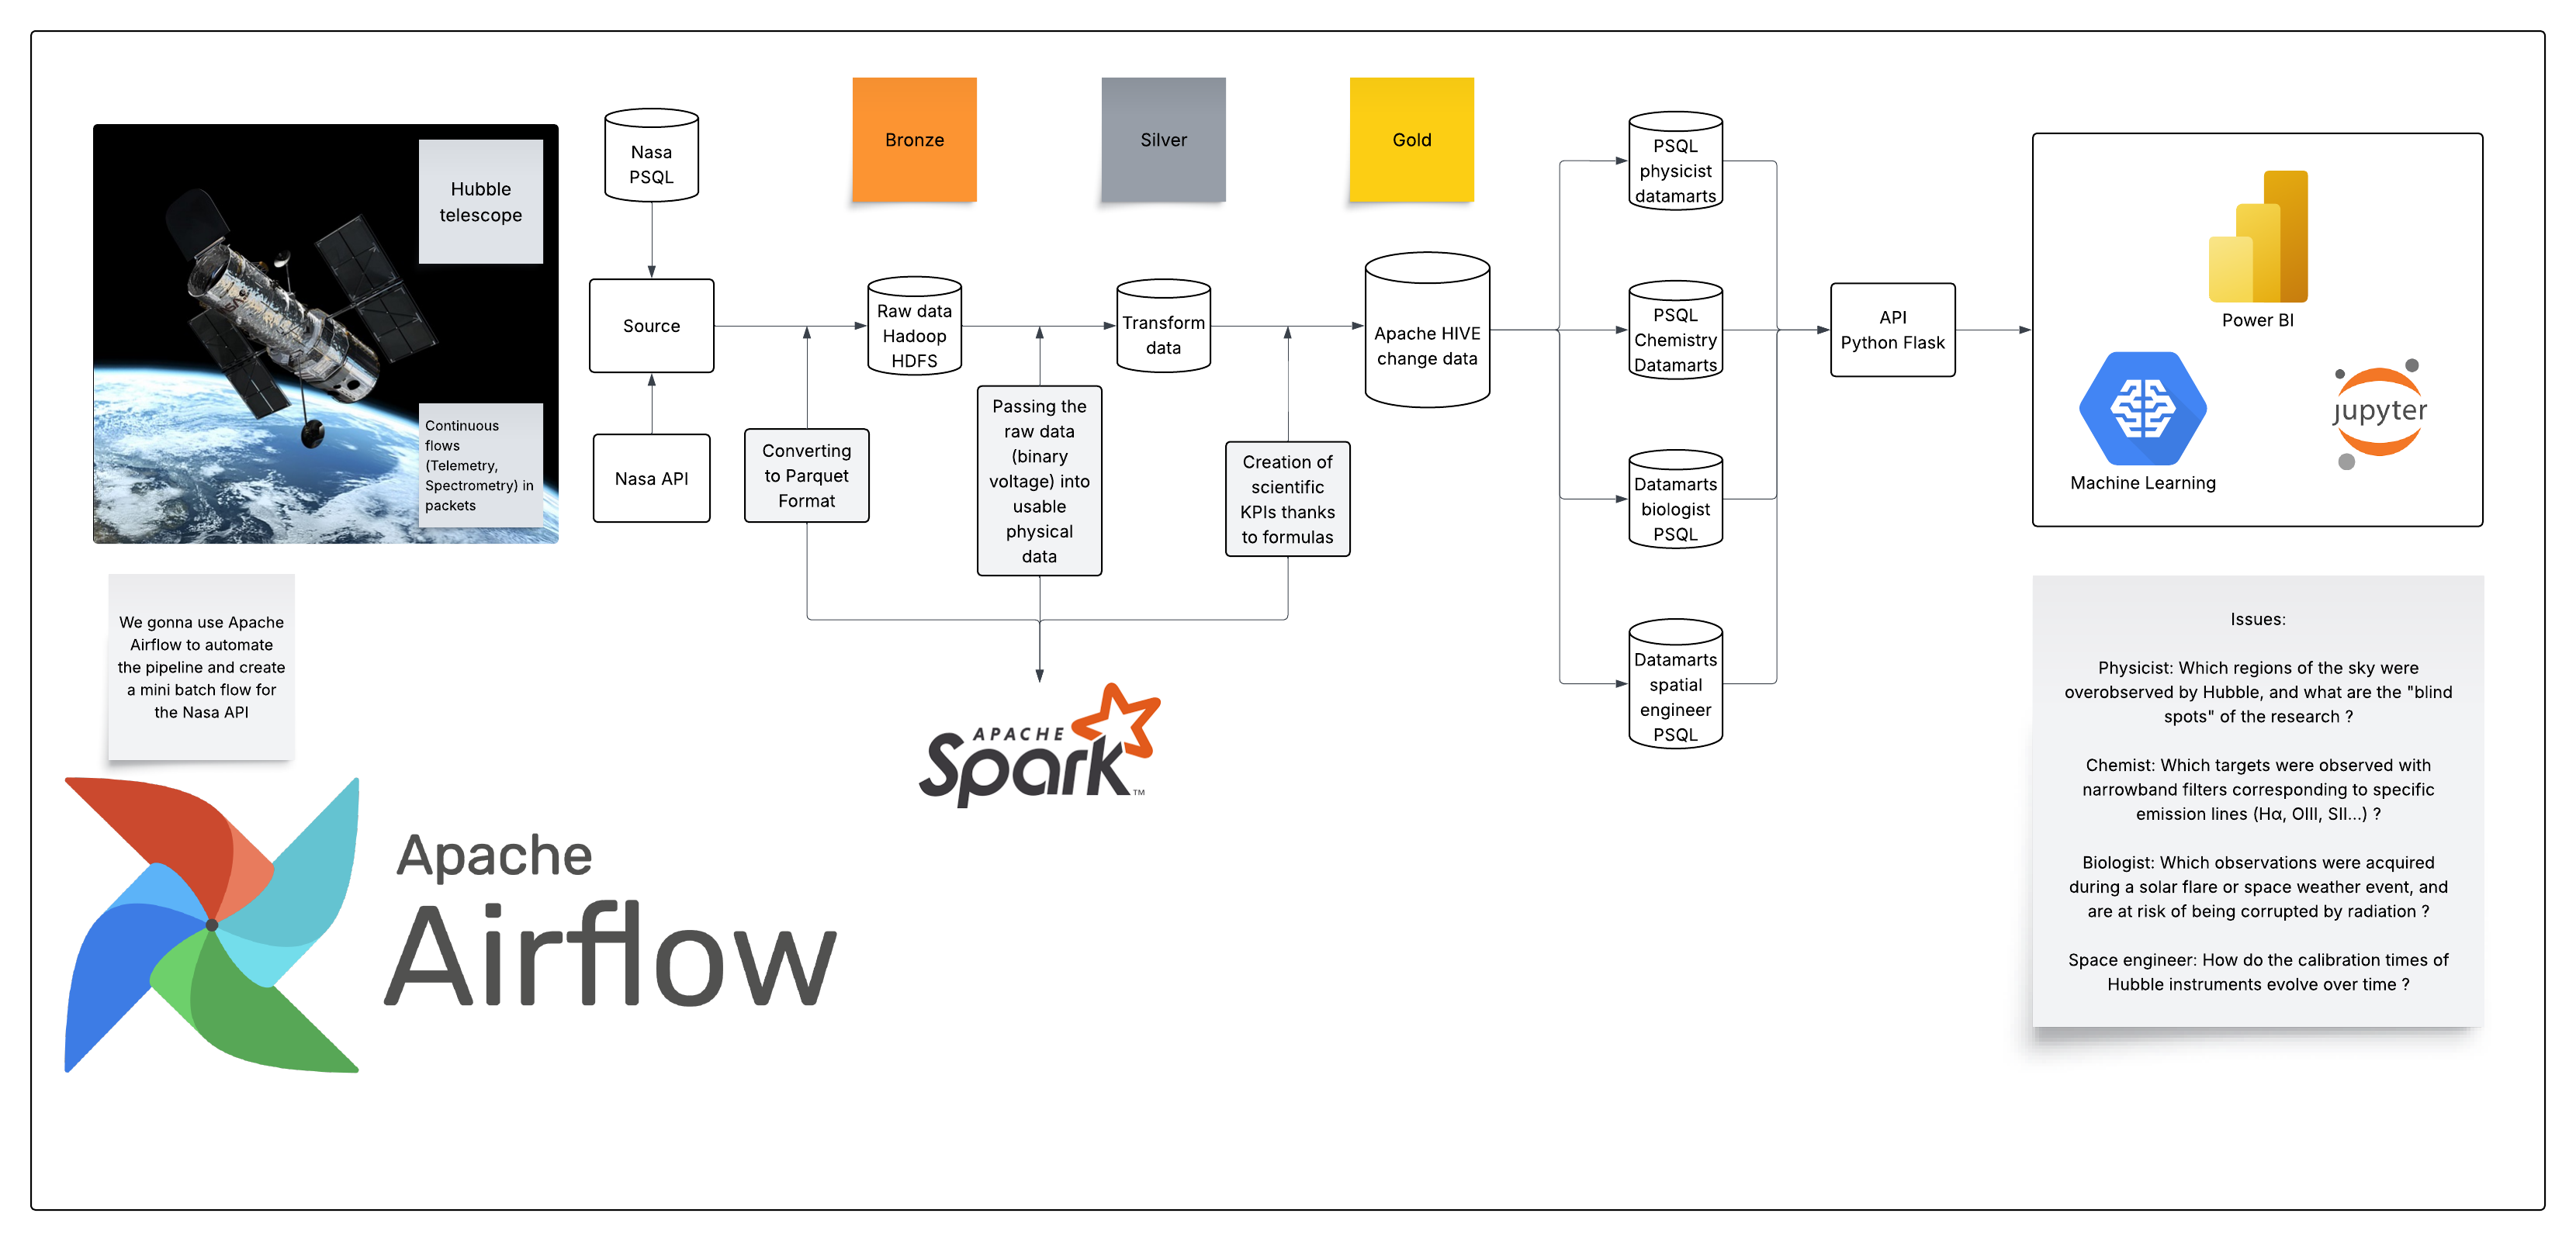
\includegraphics[width=\linewidth]{architecture.png}
    \caption{Architecture Lakehouse du projet.}
    \label{fig:archi}
\end{figure}

\subsection{Briques techniques}

L'architecture s'appuie sur les composants suivants :

\begin{itemize}
    \item \textbf{PostgreSQL} : table source MAST en entrée, datamarts métier en sortie ;
    \item \textbf{HDFS} : stockage distribué des couches Bronze, Silver et Gold au format Parquet ;
    \item \textbf{Apache Spark} : ingestion NOAA SWPC (batch et streaming) et transformations Bronze $\rightarrow$ Silver $\rightarrow$ Gold ;
    \item \textbf{Apache Hive Metastore} : catalogue exposant les tables Gold en SQL standard ;
    \item \textbf{Apache Airflow} : orchestration des DAGs batch et streaming ;
    \item \textbf{API Flask} : exposition HTTPS des datamarts, protégée par JWT.
\end{itemize}

\newpage
% ----------- PARTIE 5 -------------
\section{Spécifications fonctionnelles}

\subsection{Ingestion}

\paragraph{MAST.} La table PostgreSQL source, alimentée au démarrage du projet à partir de l'export CSV MAST, est lue en mode batch. Un job Airflow déclenche un script Python qui extrait son contenu et le dépose dans HDFS Bronze au format Parquet.

\paragraph{NOAA SWPC.} Les endpoints JSON sont interrogés en mini-batch toutes les minutes. Un job Spark Structured Streaming lit les réponses HTTP et les écrit dans HDFS Bronze au format Parquet.

\subsection{Transformations par couche}

\paragraph{Bronze $\rightarrow$ Silver.} Spark lit les fichiers Parquet bruts (MAST issu du dump PostgreSQL, archives et flux temps réel SWPC) et applique le typage des colonnes, le parsing des champs structurés (filtres, polygones, dates MJD vers UTC\dots) et la suppression des colonnes redondantes. Les apports archives et temps réel SWPC sont fusionnés et dédupliqués sur la clé temporelle pour produire une vue continue des indicateurs de météo spatiale. Les tables Silver sont écrites en Parquet sur HDFS, sans déclaration dans un catalogue.

\paragraph{Silver $\rightarrow$ Gold.} Spark SQL agrège les tables Silver pour produire les indicateurs métier des quatre datamarts. Les résultats sont écrits en Parquet sur HDFS et déclarés comme tables externes dans le Hive Metastore.

\paragraph{Gold $\rightarrow$ Datamarts.} Un dernier job Spark SQL, déclenché par un DAG Airflow distinct, lit chaque table \texttt{gold.*} via Hive et la matérialise dans PostgreSQL via JDBC, dans des schémas distincts de celui qui héberge la table MAST source. Cette étape isole la couche analytique (Hive) de la couche de service (Postgres), permettant à l'API de répondre sans dépendance à Spark.

\subsection{Datamarts}

Quatre datamarts PostgreSQL sont produits, un par profil utilisateur.

\paragraph{Physicien.} Savoir quelles régions du ciel Hubble a beaucoup observées, et lesquelles sont restées dans l'ombre.

\paragraph{Chimiste.} Retrouver les images prises à travers des filtres capables de révéler certains gaz dans l'espace, comme l'hydrogène, l'oxygène ou le soufre.

\paragraph{Biologiste.} Repérer les observations prises pendant une éruption solaire, qui risquent d'être abîmées par les radiations.

\paragraph{Ingénieur spatial.} Suivre l'usure des instruments de Hubble en regardant comment leur temps de calibration évolue au fil des années.

\subsection{Restitution}

Les quatre tables PostgreSQL sont exposées par une API REST écrite en Python avec Flask, accessible à l'adresse \href{https://efrei-bigdata-api.valentin-massonniere.ch}{https://efrei-bigdata-api.valentin-massonniere.ch}. Chaque datamart correspond à un endpoint dédié, qui retourne les enregistrements au format JSON. L'accès est protégé par jeton JWT : chaque requête doit présenter un token valide dans son en-tête \texttt{Authorization}. Les outils de visualisation et les scripts d'analyse consomment ces endpoints, sans accès direct à la base.

\newpage
% ----------- PARTIE 6 -------------
\section{Spécifications techniques}

\subsection{Volumétrie}

L'export MAST représente environ 500\,000 observations, soit quelques centaines de méga-octets en Parquet. Le flux NOAA SWPC ajoute quelques kilo-octets par minute.

\subsection{Orchestration}

Apache Airflow pilote l'ensemble du pipeline via deux DAGs complémentaires.

\paragraph{\texttt{full\_pipeline}.} DAG manuel de backfill, déclenché ponctuellement (notamment au démarrage du projet). Il rétrocharge les archives NOAA SWPC sur la fenêtre voulue, ingère la table MAST source vers Silver, déduplique les apports SWPC, puis enchaîne pour chaque profil utilisateur les étapes Gold et la matérialisation du datamart en PostgreSQL. Le datamart Biologiste dépend des deux Silver (MAST et SWPC) ; les trois autres ne dépendent que de Silver MAST.

\paragraph{\texttt{streaming}.} DAG planifié toutes les dix minutes. Il interroge les endpoints temps réel NOAA SWPC, met à jour Silver SWPC, recalcule la table Gold Biologiste et republie le datamart correspondant en PostgreSQL. C'est ce DAG qui maintient le datamart Biologiste à jour entre deux exécutions complètes du pipeline.

\subsection{Qualité et reprise}

Chaque couche est idempotente : un retraitement ne crée pas de doublons. Les enregistrements rejetés (champs manquants, valeurs incohérentes) sont conservés dans une table de rejet par couche.

\subsection{Bonus --- déploiement conteneurisé}

En complément du périmètre commun, Valentin déploie le pipeline sur un VPS personnel. Chaque composant est conteneurisé avec Docker et orchestré par Kubernetes.

Les logs des jobs sont centralisés et consultables depuis le dashboard Airflow, accessible à l'adresse \href{https://efrei-bigdata-airflow.valentin-massonniere.ch}{https://efrei-bigdata-airflow.valentin-massonniere.ch} (utilisateur \texttt{invit}, mot de passe \texttt{inviter123}). Pour des raisons de sécurité du VPS, ce compte dispose d'un accès en lecture seule et ne peut pas déclencher de DAG manuellement.

\newpage
% ----------- PARTIE 7 -------------
\section{Modèle de données}

Chaque profil utilisateur est servi par une table PostgreSQL dédiée, alimentée par un job Spark SQL depuis la couche Silver. Les schémas des sources sont documentés ci-dessous :

\subsection{Datamart Physicien}

{\small\textit{Quelles régions du ciel ont été sur-observées par Hubble, et quels sont les angles morts de la recherche~?}}

\begin{tabularx}{\linewidth}{llX}
\toprule
\textbf{Colonne} & \textbf{Type} & \textbf{Description} \\
\midrule
\texttt{ra\_bin}        & float & Position est-ouest dans le ciel (sorte de longitude céleste). \\
\texttt{dec\_bin}       & float & Position nord-sud dans le ciel (sorte de latitude céleste). \\
\texttt{nb\_obs}        & int   & Nombre de fois où cette zone du ciel a été photographiée. \\
\texttt{total\_exptime} & float & Temps total passé à observer cette zone, en secondes. \\
\bottomrule
\end{tabularx}

\subsection{Datamart Chimiste}

{\small\textit{Quelles cibles ont été observées avec des filtres à bande étroite correspondant à des raies d'émission spécifiques (H$\alpha$, OIII, SII\dots)~?}}

\begin{tabularx}{\linewidth}{llX}
\toprule
\textbf{Colonne} & \textbf{Type} & \textbf{Description} \\
\midrule
\texttt{target\_name}   & string & Nom de l'objet observé (étoile, nébuleuse, galaxie\dots). \\
\texttt{filter}         & string & Filtre coloré placé devant l'instrument pendant la prise. \\
\texttt{emission\_line} & string & Gaz que ce filtre permet de mettre en évidence (hydrogène, oxygène, soufre\dots). \\
\texttt{nb\_obs}        & int    & Nombre d'observations correspondantes. \\
\bottomrule
\end{tabularx}

\subsection{Datamart Biologiste}

{\small\textit{Quelles observations ont été acquises pendant une éruption solaire ou un événement de météo spatiale, et risquent d'être corrompues par les radiations~?}}

\begin{tabularx}{\linewidth}{llX}
\toprule
\textbf{Colonne} & \textbf{Type} & \textbf{Description} \\
\midrule
\texttt{obs\_id}      & string    & Référence unique de l'observation. \\
\texttt{t\_start}     & timestamp & Date et heure du début de la prise. \\
\texttt{t\_end}       & timestamp & Date et heure de fin de la prise. \\
\texttt{flare\_class} & string    & Intensité de l'éruption solaire qui a eu lieu pendant la prise. \\
\texttt{risk\_score}  & int       & Niveau de risque que l'image soit abîmée par les radiations. \\
\bottomrule
\end{tabularx}

\subsection{Datamart Ingénieur}

{\small\textit{Comment évoluent les temps de calibration des instruments Hubble au fil du temps~?}}

\begin{tabularx}{\linewidth}{llX}
\toprule
\textbf{Colonne} & \textbf{Type} & \textbf{Description} \\
\midrule
\texttt{instrument}       & string & Nom de l'instrument de Hubble (caméra, spectrographe\dots). \\
\texttt{year\_month}      & date   & Mois auquel la mesure correspond. \\
\texttt{avg\_calib\_time} & float  & Temps moyen passé à régler l'instrument ce mois-là, en secondes. \\
\texttt{trend\_12m}       & float  & Évolution sur les 12 derniers mois ; une valeur positive signifie que l'instrument met de plus en plus de temps à se régler. \\
\bottomrule
\end{tabularx}

\newpage
% ----------- PARTIE 8 -------------
\section{Répartition des tâches}

Le projet est mené en binôme. La répartition s'appuie sur les appétences techniques de chacun.

\subsection{Valentin}

\begin{itemize}
    \item Mise en place et maintenance du dépôt GitHub.
    \item Déploiement de l'infrastructure (HDFS, Spark, Hive, PostgreSQL, Airflow) sur un VPS personnel via Docker et Kubernetes (bonus).
    \item Ingestion du flux NOAA SWPC via Spark Structured Streaming.
    \item Transformations Silver et Gold liées aux événements de météo spatiale.
    \item Datamarts Biologiste et Ingénieur.
    \item Coordination générale du projet.
\end{itemize}

\subsection{Kevin}

\begin{itemize}
    \item Ingestion batch de l'export MAST via Python et Airflow.
    \item Transformations Silver des observations Hubble (typage, parsing des filtres, conversion MJD vers UTC\dots).
    \item Modélisation des tables Hive de la couche Silver.
    \item Datamarts Physicien et Chimiste.
\end{itemize}

\subsection{Tâches communes}

\begin{itemize}
    \item Choix techniques structurants (formats, schémas Gold, conventions de nommage).
    \item Rédaction du rapport.
\end{itemize}

\newpage
% ----------- PARTIE 9 -------------
\section{Détail des livrables}

\subsection{Dépôt GitHub}

Le dépôt est hébergé à l'adresse \href{https://github.com/TheValll/efrei-projet-big-data}{github.com/TheValll/efrei-projet-big-data} et miroiré sur GitLab pour la pipeline CI/CD. Il regroupe l'ensemble des artefacts du projet, organisés comme ceci :

\begin{itemize}
    \item \texttt{ingestion/} : export CSV MAST et script Python de chargement vers la table PostgreSQL source ;
    \item \texttt{spark/} : jobs Spark d'ingestion NOAA SWPC (archives et temps réel) et de transformation Silver $\rightarrow$ Gold $\rightarrow$ datamart pour chaque profil ;
    \item \texttt{dags/} : DAGs Airflow \texttt{full\_pipeline} (backfill manuel) et \texttt{streaming} (rafraîchissement Biologiste toutes les dix minutes) ;
    \item \texttt{api/} : API Flask en MVC (\texttt{controllers/}, \texttt{models/}, \texttt{app.py}) exposant les datamarts ;
    \item \texttt{bruno/} : collection Bruno prête à l'emploi (environnements local et prod, login et endpoints datamarts) ;
    \item \texttt{infra/} : Dockerfiles (Airflow, API, Spark, Hive Metastore), configurations Hadoop / Hive / Postgres, et manifeste Kubernetes \texttt{k8s.yaml} ;
    \item \texttt{dumps/} : dump SQL de la base \texttt{datamart} pour rejouer un état local ;
    \item \texttt{docs/} : rapport \LaTeX{} et documentation technique complémentaire ;
    \item \texttt{docker-compose.yml}, \texttt{Makefile}, \texttt{.gitlab-ci.yml}, \texttt{README.md} : stack locale, raccourcis (\texttt{make up/down/dump/restore}), pipeline CI/CD et guide de démarrage.
\end{itemize}

\subsection{Rapport}

Ce document intègre le cahier des charges et sera complété au fil du projet par :

\begin{itemize}
    \item l'architecture finale réellement implémentée ;
    \item les choix techniques et leurs justifications ;
    \item les résultats obtenus pour chaque datamart, avec exemples ;
    \item les difficultés rencontrées et les pistes d'amélioration.
\end{itemize}

\newpage
% ----------- PARTIE 10 -------------
\section{Explication technique}

Cette section détaille l'implémentation concrète du projet, depuis la stack locale jusqu'au déploiement en production.

\subsection{Stack locale et reproductibilité}

L'intégralité du projet tourne en local via un seul fichier \texttt{docker-compose.yml}, sans dépendance à un cluster ou à un service managé. Huit services y sont déclarés : PostgreSQL, le NameNode et un DataNode HDFS, un service de bootstrap PostgreSQL, le Hive Metastore, un master et un worker Spark, Airflow et l'API Flask.

\paragraph{Images.} Quatre images sont construites à partir du dossier \texttt{infra/} : \texttt{Dockerfile.airflow} (Airflow 3.0 avec client Spark et providers), \texttt{Dockerfile.api} (API Flask servie par Gunicorn), \texttt{Dockerfile.spark} (Spark 3.5 avec connecteurs Postgres et Hadoop) et \texttt{Dockerfile.hive-metastore} (Hive Metastore standalone). Les autres composants utilisent des images publiques : \texttt{postgres:16} et les images Hadoop \texttt{bde2020/hadoop-namenode} et \texttt{bde2020/hadoop-datanode}.

\paragraph{Bootstrap PostgreSQL.} Une instance PostgreSQL unique héberge à la fois les métadonnées Airflow, le metastore Hive, la table source MAST et les datamarts. Au premier démarrage, un service \texttt{postgres-bootstrap} idempotent exécute un script Bash qui crée les rôles \texttt{airflow} et \texttt{hive} ainsi que les quatre bases \texttt{airflow\_metadata}, \texttt{nasa\_db\_raw} (table source MAST), \texttt{datamart} (datamarts Gold) et \texttt{hive\_metastore}. Les autres services attendent sa terminaison via \texttt{depends\_on} avec la condition \texttt{service\_completed\_successfully}.

\paragraph{Persistance et réseau.} Trois volumes nommés (\texttt{postgres-data}, \texttt{hadoop-namenode}, \texttt{hadoop-datanode}) garantissent la persistance des données entre redémarrages. Les services communiquent sur le réseau Docker par défaut, en utilisant les noms de services comme noms d'hôtes (\texttt{postgres}, \texttt{namenode}, \texttt{spark-master}, \texttt{hive-metastore}\dots). Les UIs sont exposées sur l'hôte : Airflow sur \texttt{8080}, Spark sur \texttt{8081}, HDFS NameNode sur \texttt{9870}, API sur \texttt{5000} et PostgreSQL sur \texttt{5432}.

\paragraph{Configuration par variables d'environnement.} Tous les paramètres sensibles (mots de passe Postgres, Airflow, API, secret JWT) sont injectés depuis un fichier \texttt{.env} non versionné. Un \texttt{.env.example} fournit des valeurs de développement par défaut et documente les clés attendues.

\paragraph{Makefile.} Quatre cibles couvrent le cycle de vie local : \texttt{make up} (build et démarrage de la stack), \texttt{make down} (arrêt sans suppression des volumes), \texttt{make dump} (export de la base \texttt{datamart} vers \texttt{dumps/datamart.sql}) et \texttt{make restore} (rejeu d'un dump local).

\subsection{Jobs Spark}

Le dossier \texttt{spark/} regroupe douze scripts PySpark répartis en quatre étapes : ingestion NOAA SWPC vers Bronze, Bronze $\rightarrow$ Silver, Silver $\rightarrow$ Gold et Gold $\rightarrow$ datamart PostgreSQL.

\paragraph{Ingestion NOAA SWPC vers Bronze.} Deux scripts (live et archive) écrivent dans le même répertoire Bronze sous un schéma unifié (\texttt{endpoint}, \texttt{event\_time}, \texttt{record}, \texttt{ingested\_at}) et appliquent la même stratégie de fusion : union avec l'existant puis déduplication par fenêtre sur \texttt{(endpoint, event\_time)}. Le live interroge quatre endpoints JSON (Kp, X-ray, vent solaire, éruptions) ; l'archive parse les rapports texte annuels GOES X-Ray.

\paragraph{Bronze $\rightarrow$ Silver.} \texttt{silver\_mast.py} lit la table source via JDBC, type les colonnes et convertit les dates MJD en \texttt{timestamp} UTC. \texttt{silver\_noaa.py} parse le JSON Bronze, extrait la classe X-ray par \textit{regex} et déduplique les apports archives et live sur \texttt{(event\_start, xray\_class)}.

\paragraph{Silver $\rightarrow$ Gold.} Les quatre jobs déclarent les tables externes Silver dans Hive, exécutent une requête Spark SQL d'agrégation et publient le résultat comme table externe \texttt{gold.*}. Les spécificités métier :

\begin{itemize}
    \item \textbf{Physicien} : binning du ciel par degré (\texttt{FLOOR} sur \texttt{s\_ra}, \texttt{s\_dec}) ;
    \item \textbf{Chimiste} : jointure avec une table de référence des filtres à bande étroite ;
    \item \textbf{Biologiste} : jointure d'intervalles temporels MAST $\times$ éruptions, calcul d'un \texttt{risk\_score} dérivé de la classe X-ray ;
    \item \textbf{Ingénieur} : agrégation mensuelle par instrument sur les observations de calibration, tendance via \texttt{LAG} sur 12 mois.
\end{itemize}

\paragraph{Gold $\rightarrow$ datamart.} Les quatre scripts \texttt{datamart\_*.py} lisent chacun leur table \texttt{gold.*} via Hive et l'écrivent en \texttt{overwrite} dans la base \texttt{datamart} via JDBC.

\subsection{API Flask}

L'API est servie par Gunicorn et organisée en MVC : \texttt{app.py} (factory et configuration), \texttt{controllers/} (blueprints HTTP) et \texttt{models/} (requêtes SQL). Trois blueprints sont enregistrés : \texttt{/health}, \texttt{/auth} et \texttt{/datamarts}.

\paragraph{Authentification.} \texttt{/auth/login} compare les identifiants envoyés à deux comptes (\texttt{admin}, \texttt{viewer}) configurés par variables d'environnement, puis émet un \texttt{access\_token} (1\,h) et un \texttt{refresh\_token} (7\,j) via \textit{flask-jwt-extended}. \texttt{/auth/refresh} renouvelle l'\texttt{access\_token} à partir du refresh.

\paragraph{Endpoints datamarts.} Quatre routes \texttt{GET /datamarts/\{profil\}} renvoient les lignes du datamart correspondant en JSON. Toutes sont protégées par \texttt{@jwt\_required()} et acceptent une pagination \texttt{limit} / \texttt{offset} ; les profils Biologiste et Ingénieur acceptent en plus un filtre temporel \texttt{from} / \texttt{to}.

\paragraph{Accès PostgreSQL.} Les modèles utilisent un pool psycopg2 (\texttt{DBPool}) initialisé au démarrage avec \texttt{DATAMART\_DSN}, et un curseur \texttt{RealDictCursor} pour sérialiser directement en JSON. Une collection Bruno (\texttt{bruno/}) fournit les requêtes prêtes à l'emploi pour les environnements local et prod.

\subsection{Déploiement Kubernetes}

L'ensemble de la stack est redéployé sur un cluster Kubernetes hébergé sur un VPS personnel, dans le namespace \texttt{efrei-big-data}. Le fichier \texttt{infra/k8s.yaml} regroupe l'intégralité des ressources : huit \texttt{Deployment} (Postgres, Airflow, API, NameNode, DataNode, Spark master, Spark worker, Hive Metastore), leurs \texttt{Service} associés, trois \texttt{PersistentVolumeClaim} pour les données persistantes et un \texttt{ConfigMap} d'initialisation Postgres.

\paragraph{Images.} Les images custom (Airflow, API, Spark, Hive Metastore) sont tirées depuis le registry GitLab via un \texttt{imagePullSecret regcred}. Postgres et Hadoop utilisent les mêmes images publiques qu'en local.

\paragraph{Secrets.} Un \texttt{Secret efrei-secrets} centralise les mots de passe Postgres et Airflow ; il est recréé à chaque déploiement par la pipeline CI/CD à partir de variables protégées GitLab.

\paragraph{Exposition HTTPS.} Deux \texttt{Ingress} routent \texttt{efrei-bigdata-airflow.valentin-massonniere.ch} et \texttt{efrei-bigdata-api.valentin-massonniere.ch} vers les services internes. Les certificats TLS sont émis automatiquement par \textit{cert-manager} avec l'issuer \texttt{letsencrypt-prod}.

\subsection{Pipeline CI/CD GitLab}

Le dépôt est miroiré sur GitLab pour profiter de son CI/CD intégré. Le fichier \texttt{.gitlab-ci.yml} déclare deux étapes (\texttt{build} puis \texttt{deploy}) qui ne s'exécutent que sur \texttt{main}.

\paragraph{Build.} Quatre jobs construisent en parallèle les images Airflow, API, Spark et Hive Metastore avec Docker-in-Docker, puis les poussent sur le registry GitLab sous deux tags : le SHA court du commit et \texttt{latest}.

\paragraph{Deploy.} Un job final utilise l'image \texttt{dtzar/helm-kubectl} pour reconstruire un \texttt{kubeconfig} à partir d'une variable CI/CD encodée en base64, recréer les secrets (\texttt{regcred} pour le registry, \texttt{efrei-secrets} pour les mots de passe), appliquer \texttt{infra/k8s.yaml} et déclencher un \texttt{rollout restart} sur les huit déploiements pour qu'ils retirent les nouvelles images.

\paragraph{Variables sensibles.} Mots de passe (Postgres, Airflow), \texttt{kubeconfig} et identifiants registry sont stockés en variables protégées GitLab et n'apparaissent jamais dans le dépôt ni dans les logs CI/CD.

\newpage
% ----------- PARTIE 11 -------------
\section{Visualisation des résultats via Power BI}

\newpage
% ----------- PARTIE 12 -------------
\section{Conclusion}

\newpage
\thispagestyle{empty}
\vspace*{\fill}

\begin{center}

{\large Hubble Lakehouse}\\[0.2cm]
{\small \textit{Pipeline Big Data pour l'analyse des observations du télescope spatial Hubble}}\\[1.5cm]

\rule{0.5\linewidth}{0.4pt}\\[0.6cm]

{\Large Signatures}\\[2cm]

\begin{minipage}[t]{0.4\linewidth}
\centering
\vspace{3cm}
\rule{\linewidth}{0.4pt}\\[0.3cm]
{\large Valentin Massonnière}\\[0.1cm]
{\small Efrei Paris}\\
{\small \textit{M1 Data Engineering \& AI --- DE3}}
\end{minipage}
\hfill
\begin{minipage}[t]{0.4\linewidth}
\centering
\vspace{3cm}
\rule{\linewidth}{0.4pt}\\[0.3cm]
{\large Kevin Heugas}\\[0.1cm]
{\small Efrei Paris}\\
{\small \textit{M1 Data Engineering \& AI --- DE3}}
\end{minipage}

\vspace{3cm}

{\small Fait à Paris, le \today.}

\end{center}

\vspace*{\fill}

\end{document}
